\documentclass[12pt]{report}
\usepackage[margin=1in]{geometry}
\usepackage{xcolor}
\usepackage{fontspec}
\usepackage{graphicx}
\usepackage{tabularx}
\usepackage{authoraftertitle}

\title{Criterion B: Design}
\definecolor{msblue}{HTML}{5AB5D8}
\makeatletter
\graphicspath{{images/}}
\newenvironment{code}{\ttfamily}{\par}

\begin{document}
\centerline{\textcolor{msblue}{
		\fontspec{Cambria}\textbf{\fontsize{13}{13}\MyTitle}
	}}

\section*{UML Diagram}
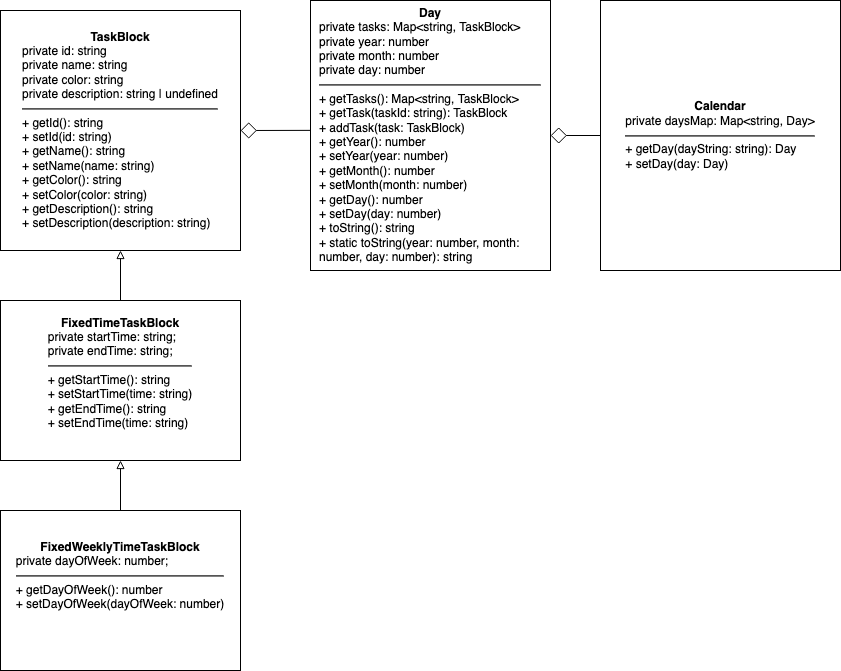
\includegraphics[width=\textwidth]{uml-diagram.png}

\section*{Flowchart}
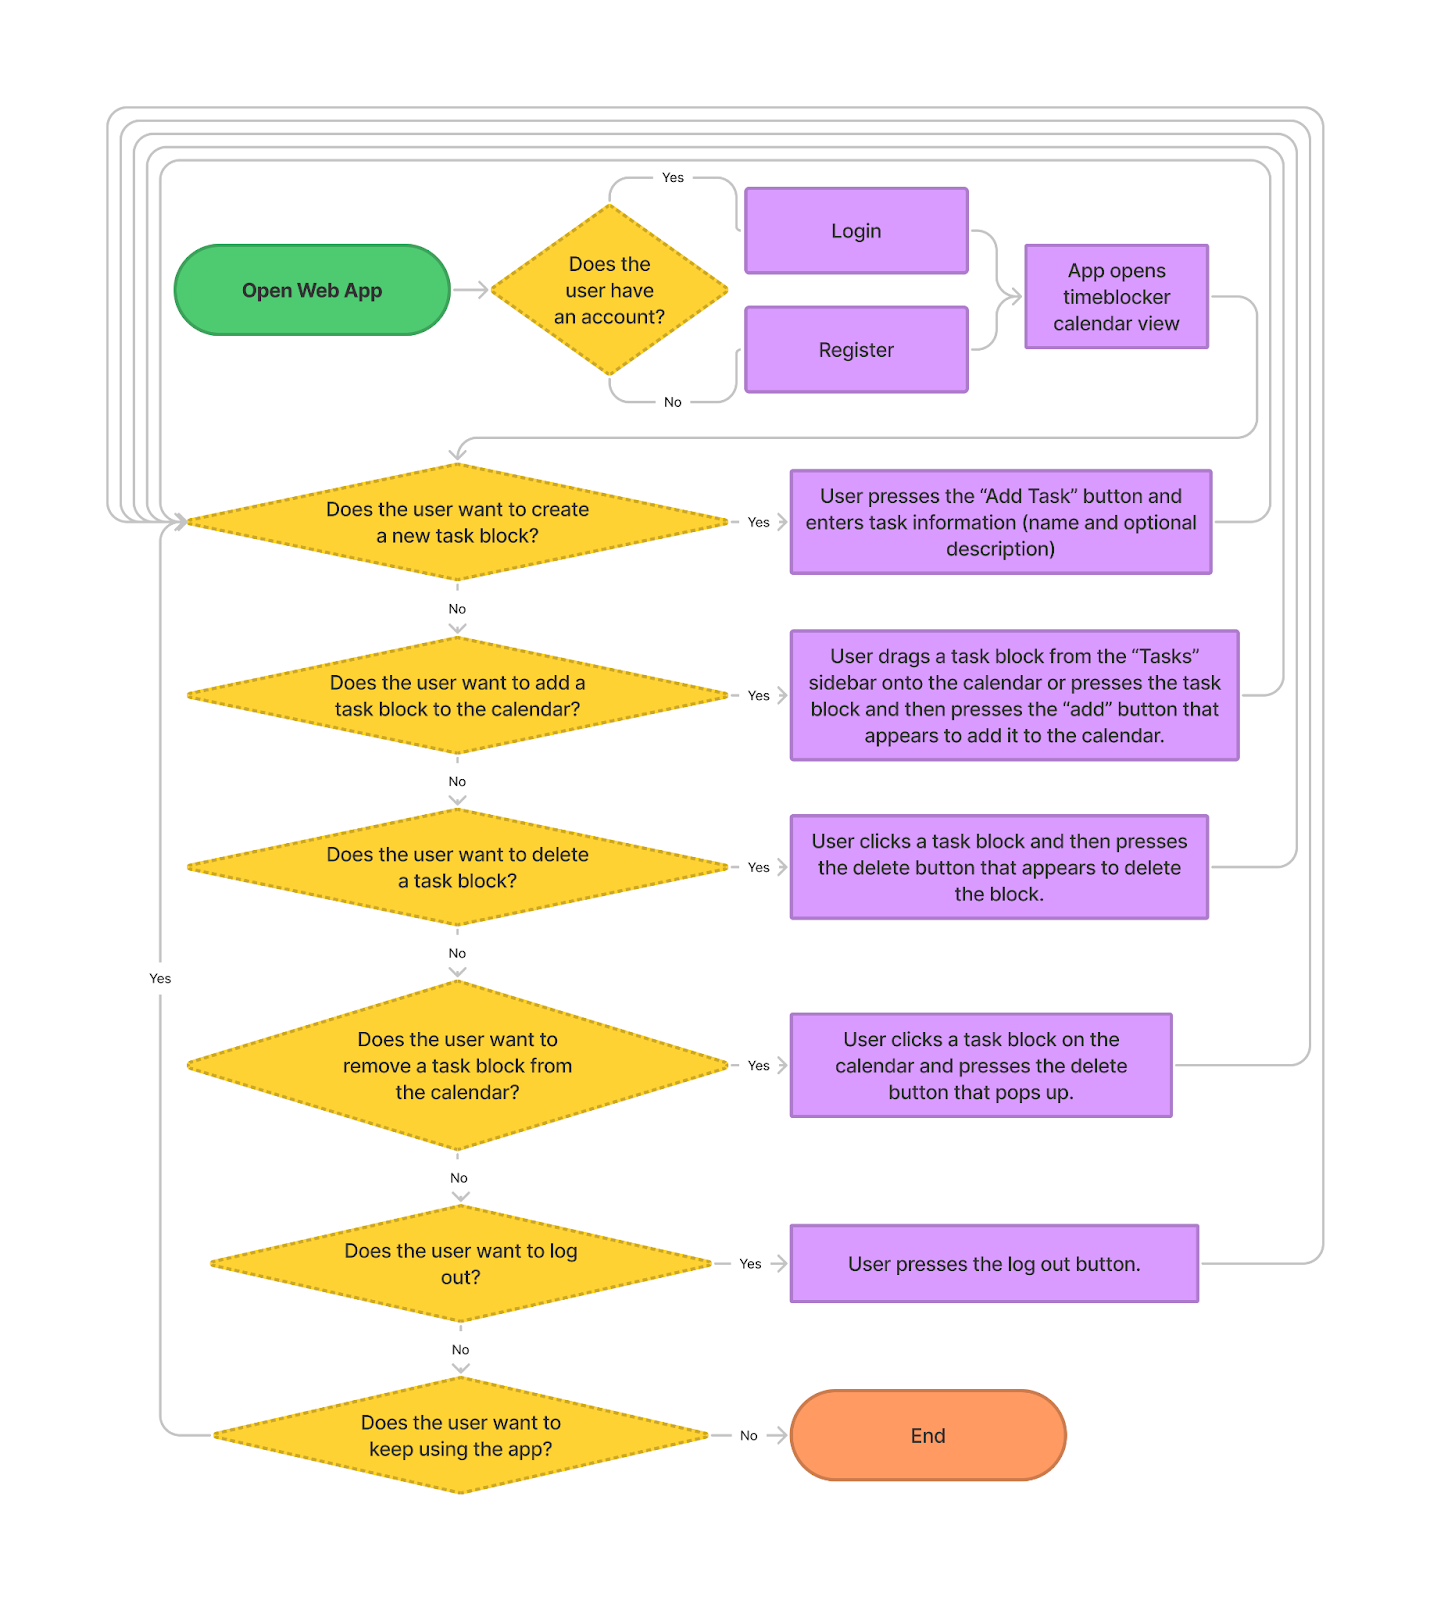
\includegraphics[width=\textwidth]{flowchart.png}

\section*{UI Design}
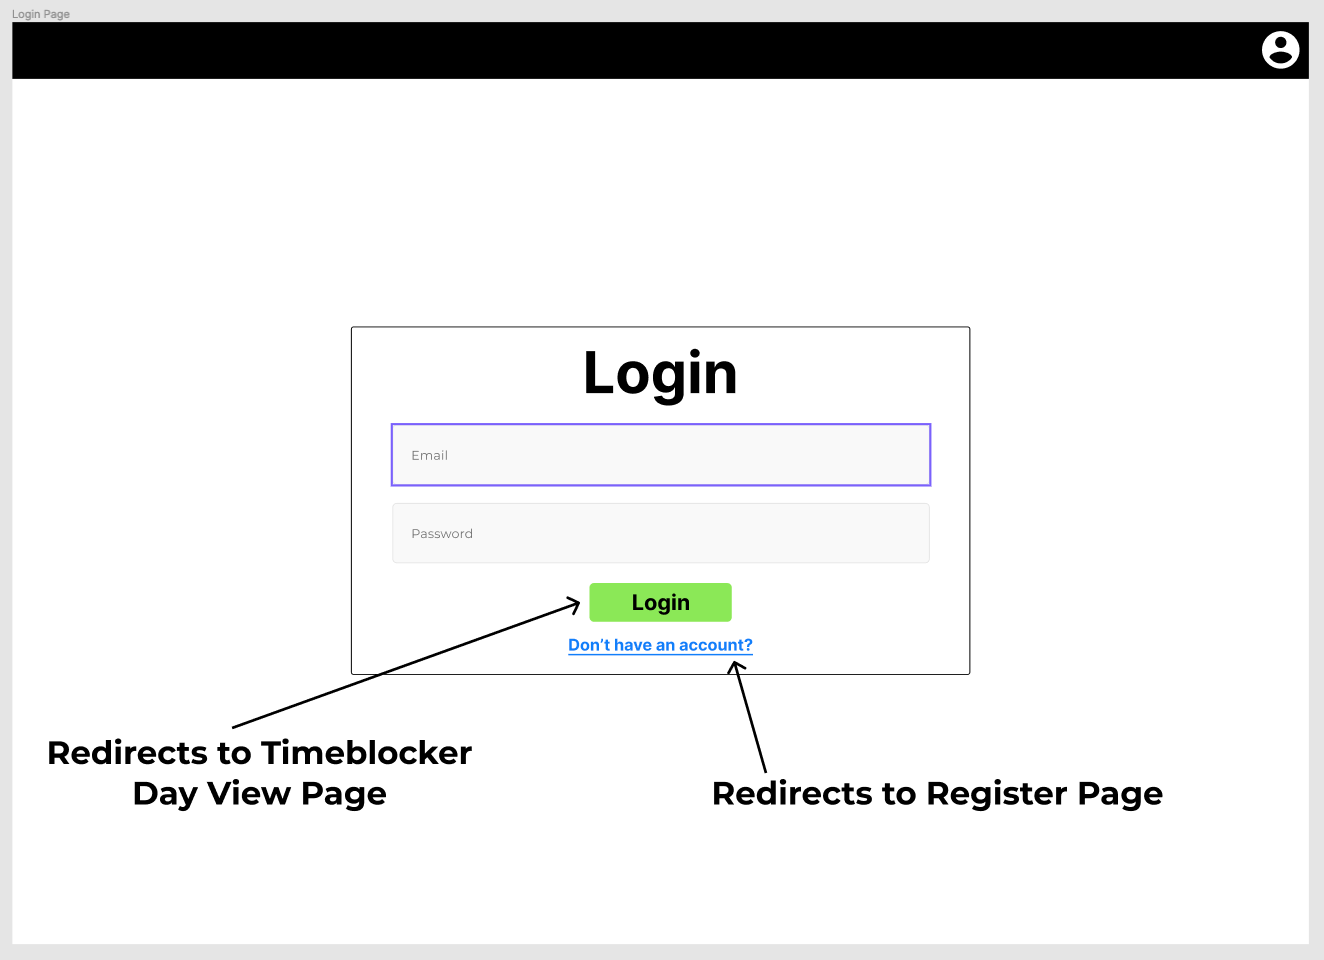
\includegraphics[width=\textwidth]{login-page.png}
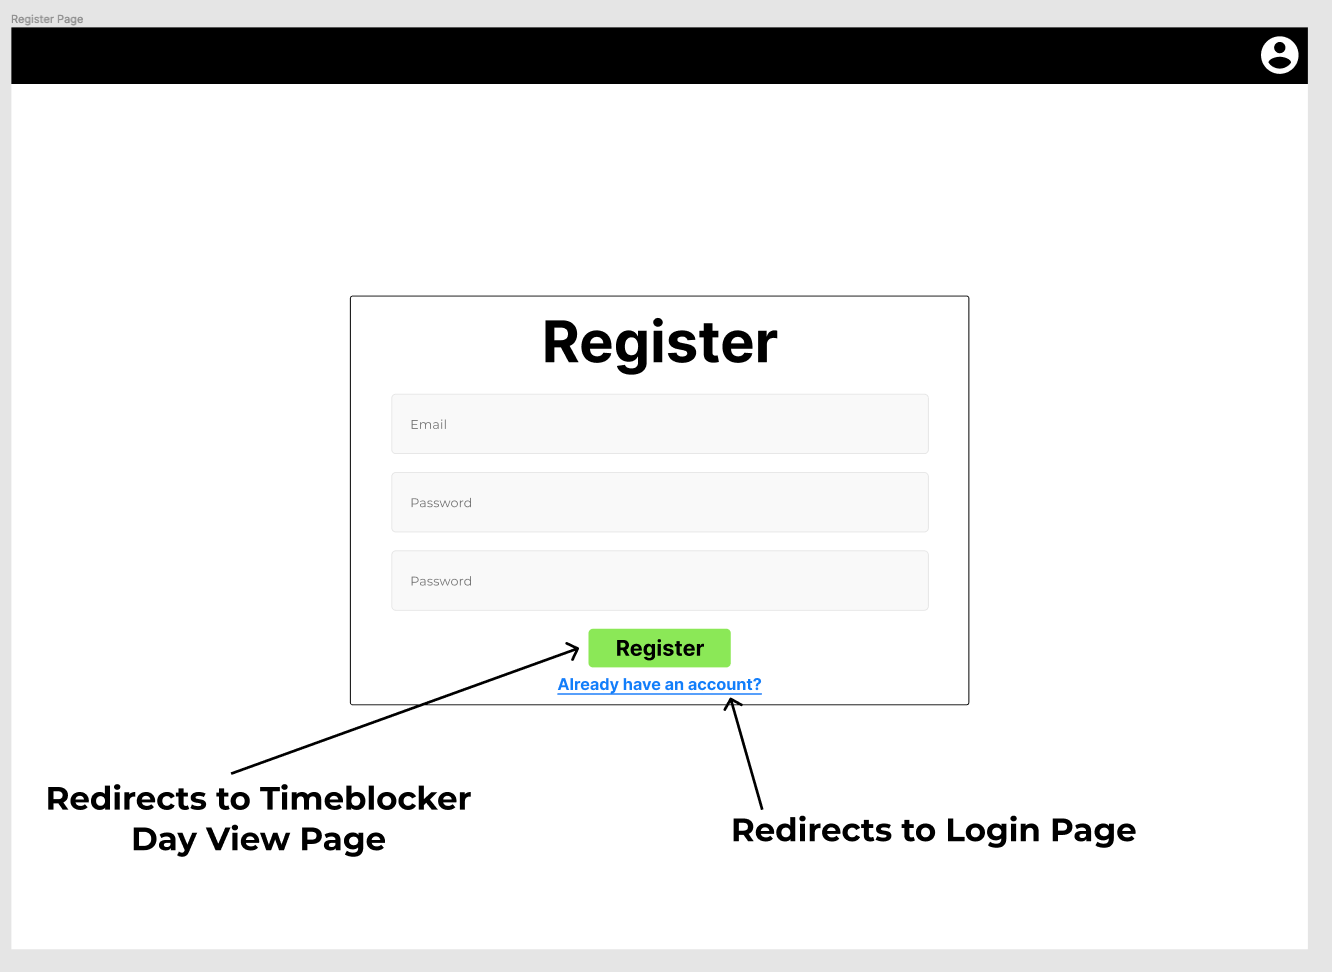
\includegraphics[width=\textwidth]{register-page.png}
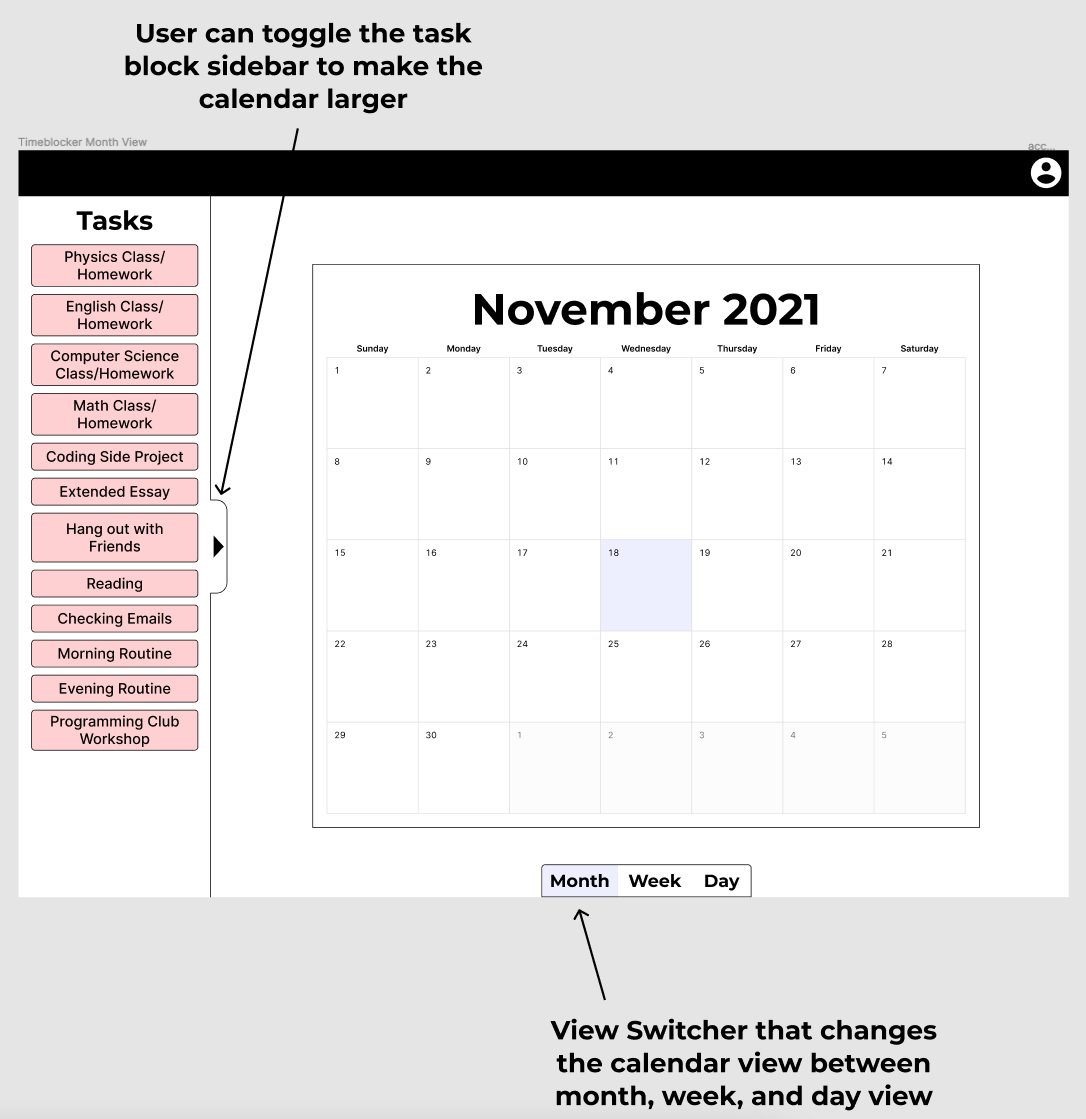
\includegraphics[width=\textwidth]{month-view.png}
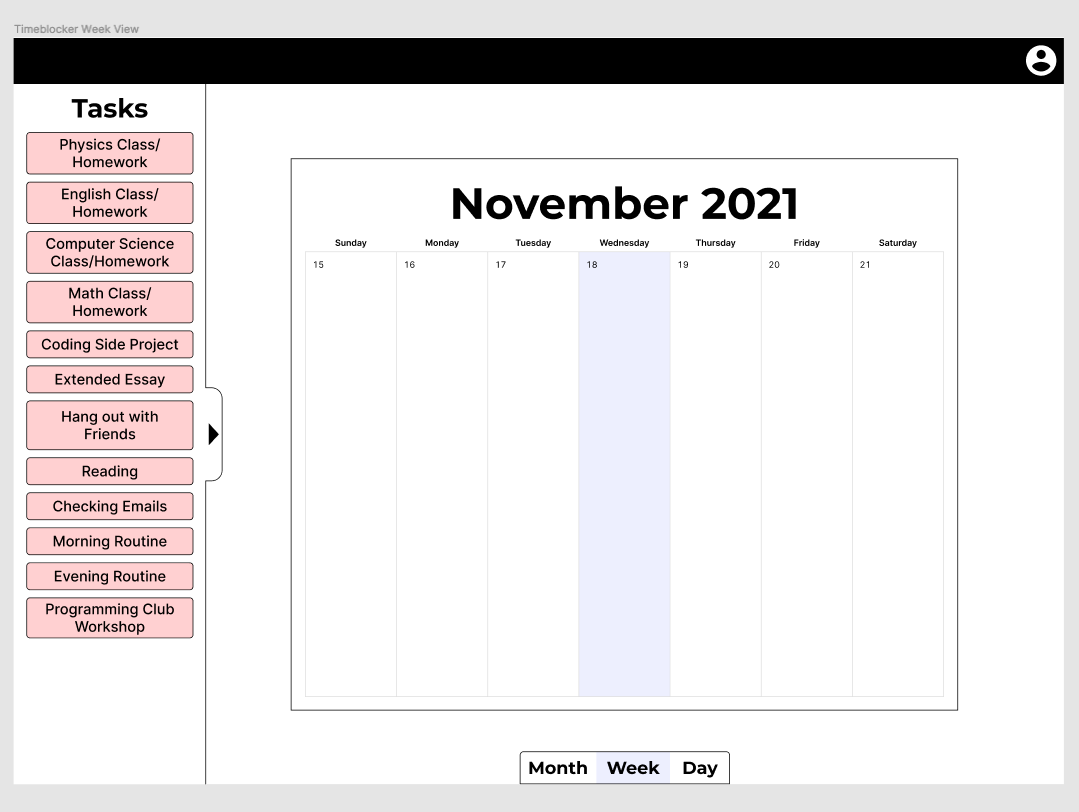
\includegraphics[width=\textwidth]{week-view.png}
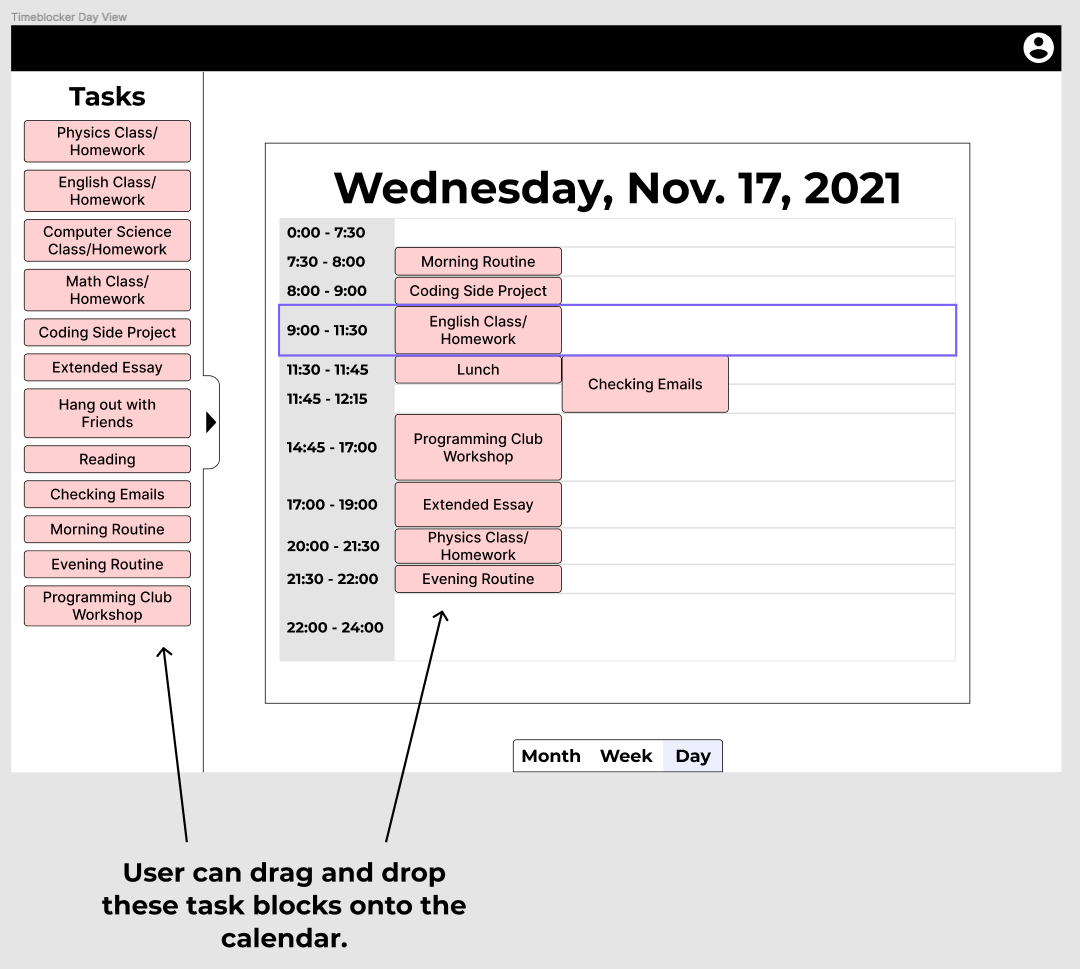
\includegraphics[width=\textwidth]{day-view.png}

\section*{Algorithms}

\subsection*{Merge Sort}
\bgroup\obeylines
\noindent\begin{code}
// The comparison function returns true if the first element is less than the second element
function merge (leftArray, rightArray, comparisonFunction)
	sortedArray = []
	leftIndex = 0
	rightIndex = 0

	while leftIndex < leftArray.length and rightIndex < rightArray.length
		// If the left element is less than the right element
		if comparisonFunction(left[leftIndex], right[rightIndex])
			sortedArray.push(left[leftIndex])
			leftIndex += 1
		else
			sortedArray.push(right[rightIndex])
			rightIndex += 1

	return sortedArray +
		remaining elements of left array +
		remaining elements of right array

function mergeSort (array, comparisonFunction)
	half = array.length / 2

	if array.length < 2
		return array

	left = array.slice(0, half)
	right = array.slice(half, array.length)

	return merge(
		mergeSort(left, comparisonFunction),
		mergeSort(right, comparisonFunction)
	)
\end{code}
\egroup

\newpage
\section*{Product Development Plan}
\def\arraystretch{1.5}
\begin{tabularx}{\textwidth}{|X|X|}
	\hline
	Function
	 & Comments
	\\\hline
	Account Entry Screens
	\begin{itemize}
		\item Login Screen
		\item Register Screen
	\end{itemize}
	\textbf{Time:} 1 week
	 &
	To synchronize the user's calendar across multiple devices, they’ll need to create and login with an account.
	However, it'll still be possible for them to use Timeblocker without an account, but the data will be saved on their machine and won’t be synced across devices.
	\\\hline
	The Task Blocks Sidebar
	\begin{itemize}
		\item Ability to create, update, and delete task blocks
		\item Sorting, filter, and categorization functions
		\item Implementing different types of task blocks
	\end{itemize}
	\textbf{Time:} 3 weeks
	 &
	The user needs to be able to manage their task blocks on the sidebar, and because they can have many tasks, they need an easy way to navigate through these tasks and categorize them.
	\\\hline
	The Calendar View
	\begin{itemize}
		\item Month, Week, and Day views
		\item Time Grid in Day View
	\end{itemize}
	\textbf{Time:} 3 weeks
	 &
	The calendar view needs to support three different view modes, the day view being the most complicated since it displays a detailed view of the user’s tasks for that day.
	The user must be able to interact with the calendar and have the ability to drag tasks around to reorder them.
	\\\hline
\end{tabularx}

\end{document}